\section{Typ Polymorphismus}
\textbf{Dynamische Typ-Bestimmung}
\begin{itemize}
    \item Typ-Deskriptor = Dynamischer Typ des Objektes
\end{itemize}
\subsection{Ancestor Tables}
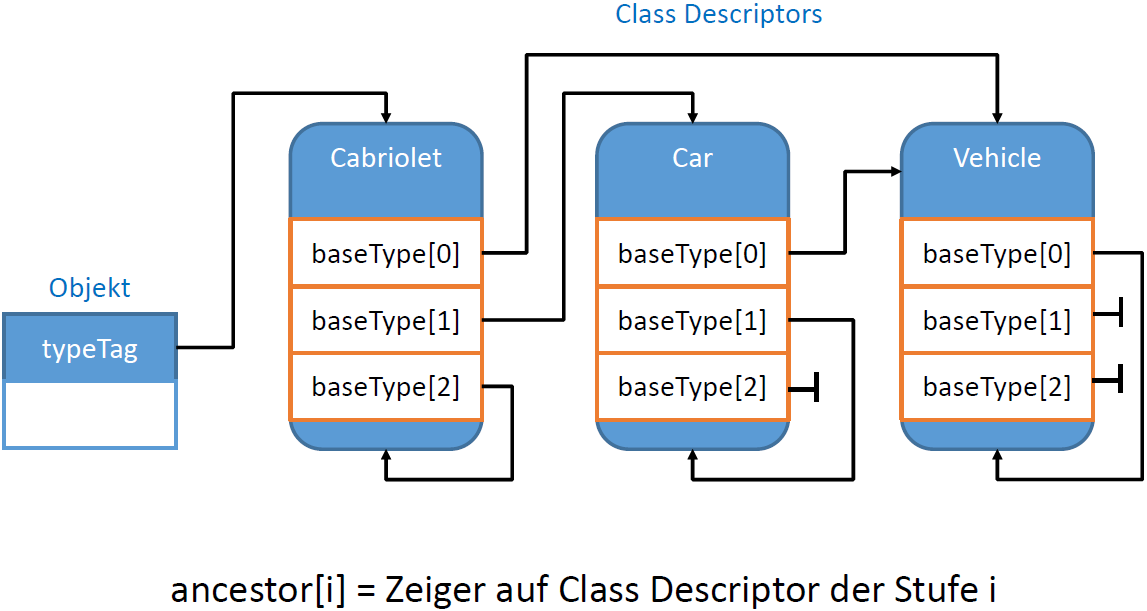
\includegraphics[width=0.6\linewidth]{ancestor_tables.png}
\subsection{Implementierung}
\begin{lstlisting}
private void instanceofTest(Object operand) {
    var instance = checkPointer(pop());
    if (instance == null) {
        push(false);
    } else {
        var targetType = checkClassDescriptor(operand);
        push(typeTest(instance, targetType));
    }
}

private void checkCast(Object operand) {
    var instance = checkPointer(pop());
    push(instance);
    var targetType = checkClassDescriptor(operand);
    if (!typeTest(instance, targetType)) {
        throw new VMException("Invalid cast");
    }
}
\end{lstlisting}

\subsection{Virtual Method Table}
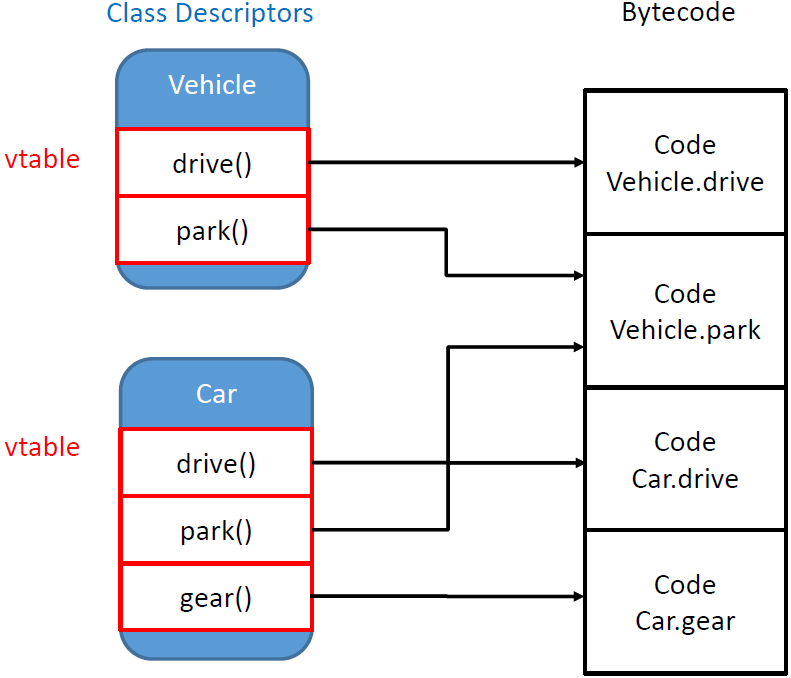
\includegraphics[width=0.4\linewidth]{virtual_method_table.png}
\subsubsection{Lineare Erweiterung}
\textbf{Jede virtuelle Methode hat einen Eintrag}
\begin{itemize}
    \item Methoden der Basisklasse oben
    \item Neu deklarierte Methoden der Subklasse unten
    \item Funktioniert nur bei Single Inheritance
\end{itemize}
\subsubsection{Method Position}
\begin{itemize}
    \item Jede virtuelle Methode hat fixe Position in vtable
    \item Position ist statisch bekannt im deklarierten Typ
\end{itemize}
\subsubsection{Method Descriptor}
\begin{itemize}
    \item Zusätzliche Indirektion über Methoden-Deskriptor
    \item Interpreter braucht Infos zu Typen von Params/Locals
\end{itemize}
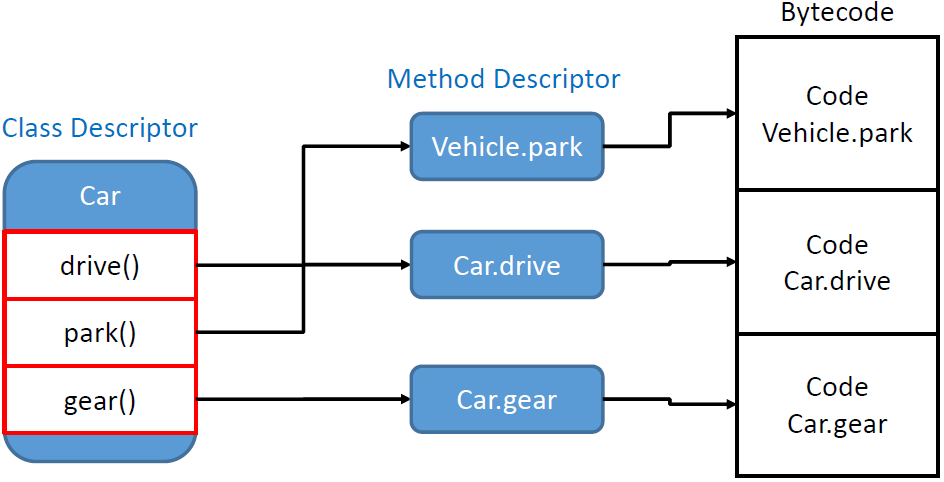
\includegraphics[width=0.5\linewidth]{method_descriptor.png}
\subsubsection{Implementation}
\begin{lstlisting}
private void invokeVirtual(Object operand) {
    var staticMethod = checkMethodDescriptor(operand);
    var parameterTypes = staticMethod.getParameterTypes();
    var arguments = new Object[parameterTypes.length];
    for (int index = arguments.length - 1; index >= 0; index--) {
        arguments[index] = pop();
        checkType(arguments[index], parameterTypes[index]);
    }
    var target = checkPointer(pop());
    invokeVirtual(staticMethod, target, arguments);
}

private void invokeVirtual(MethodDescriptor staticMethod, Pointer target, Object[] arguments) {
    if (target == null) {
        throw new VMException("Null dereferenced");
    }
    var type = checkClassDescriptor(heap.getDescriptor(target));
    var position = staticMethod.getPosition();
    var vtable = type.getVirtualTable();
    var dynamicMethod = vtable[position];
    var locals = initLocals(dynamicMethod.getLocalTypes());
    if (useJIT && jitEngine.supports(dynamicMethod)) {
        performJITCall(dynamicMethod, arguments);
    } else {
        callStack.push(new ActivationFrame(dynamicMethod, target, arguments, locals));
    }
}
\end{lstlisting}

\subsection{Interface Support}
\begin{itemize}
    \item Interfaces global durchnummerieren
    \item Pro Class Descriptor eine Interface Tabelle (itable)
    \begin{itemize}
        \item Interfaces nach Nummer = Position eintragen
    \end{itemize}
    \item Einträge in \textit{itable} verweisen auf \textit{vtable}
    \item Class Deskriptor verweist auf \textit{itable} (ibase-Pointer)
\end{itemize}
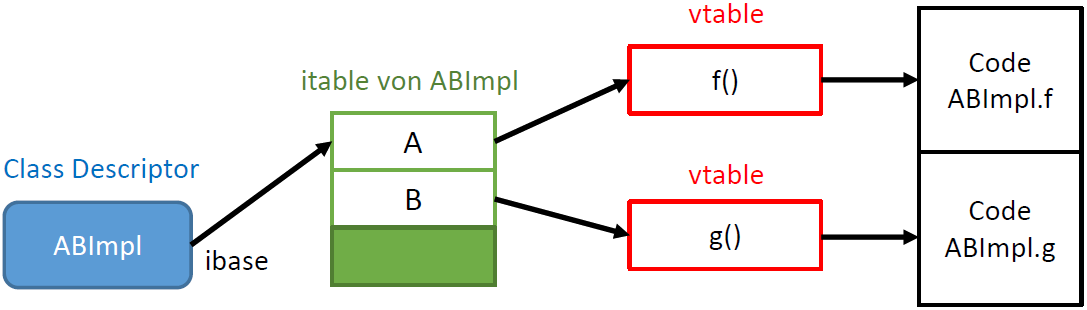
\includegraphics[width=0.6\linewidth]{interface_support.png}

\subsubsection{Verzahnte Interface Tabelle}
\textbf{Grund}
\begin{itemize}
    \item Einfache Interface Tabellen sind ein Speicherproblem
    \item Lange itables bei vielen Interfaces
    \item Viele Lücken wegen globaler Nummeriereung
\end{itemize}
\textbf{Konzept}
\begin{itemize}
    \item \textit{itables} im Speicher kollisionsfrei übereinanderlegen
    \item Muss nun prüfen, ob Eintrag für Typ gültig ist (Vermerk des Class Descriptors in \textit{vtable})
\end{itemize}
\subsubsection{Verschiedene Offsets}
\begin{itemize}
    \item Verzahnung auch mit veschiedenen Offsets möglich
\end{itemize}

\subsubsection{Gesamtbild}
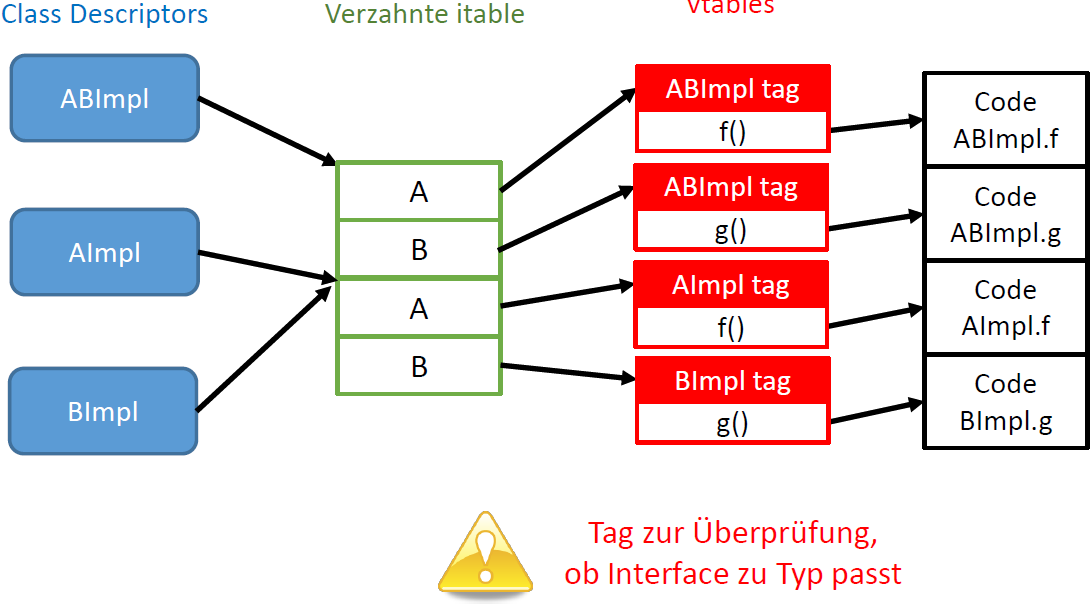
\includegraphics[width=0.6\linewidth]{gesamtbild_interface_support.png}
